The \fullsys (\sys) is the abstraction of a group of energy-harvesting battery-less sensor nodes seeking to approximate the continuous sensing availability characteristic of a battery-powered sensor. The design of a \sys needs to consider four main aspects: 
\begin{enumerate*}[label=(\roman*)]
\item how the nodes' awake time is distributed; 
\item the consequence of emulating continuous sensing availability by chaining multiple short on-times; 
\item the effect of the environment on the \sys's availability; and 
\item the spacial coverage of the event of interest, which determines the diameter of the \sys.
\end{enumerate*}

However, let us first characterize the power cycle of an energy-harvesting battery-less device. 
An energy-harvesting intermittent node frequently switches between off and on, charging energy and operating. We can characterize, from a time perspective, this charge-discharge (or power) cycle using the following notation, ($t_\text{on}$, $t_\text{p}$), where $t_\text{on}$ is the node's uptime interval, and $t_\text{p} \coloneqq t_\text{on} + t_\text{off}$, where $t_\text{off}$ is the node's charging time interval.

\subsection{Sensing}
The ability of a \sys to sense depends on the availability of its intermittent nodes and on the characteristics of the event of interest. 

\subsubsection{Coalesced availability}
\label{subSec:availability}
The \sys's availability is the projection of its underlying intermittent nodes' on-times on the time axis. 
To determine the expected availability of a \sys, the strategy being employed to distribute its nodes' on-times must be specified first.
%
\paragraph{Explicit on-time division strategy}
A \sys can build on top of the recent advancements in passive (light or RF) communication~\cite{LuzLink,liu2013ambient} and ultra-low-power timers~\cite{hester2017timely} to apply a time-division multiplexing strategy to minimize on-times overlapping. For example, a node calculates its average on-time $\overline{t_\text{on}}$ and off-time $\overline{t_\text{off}}$ for $N$ power cycles. Then, it encodes the information $({\overline{t_\text{off}}, \overline{t_\text{on}}})$ in a message and broadcasts it at the beginning of its power cycle. When a node receives this message it will have full knowledge about the transmitting node's power cycle. It can then alter its power cycle, relative to the transmitting nodes cycle, by either increasing (or decreasing) its power consumption to shorten (or lengthen) its on-time and subsequently shift its power cycle to a different time slot. 

With such explicit on-times control strategy, a \sys of $N$ nodes with on-time of $\overline{t_\text{on}}$ and off-time of $\overline{t_\text{off}}$ will have an availability $\approx N\times \frac{\overline{t_\text{on}}}{\overline{t_\text{p}}} \pmod{100\%}$. However, we expect such an approach to introduce significant overhead as a scattering algorithm~\cite{giusti2007decentralized} must be frequently executed, messages need to be exchanged, and clocks should be synchronized. Therefore, we propose a different on-time spreading strategy.  
%
\begin{figure}[t]
		\centering
		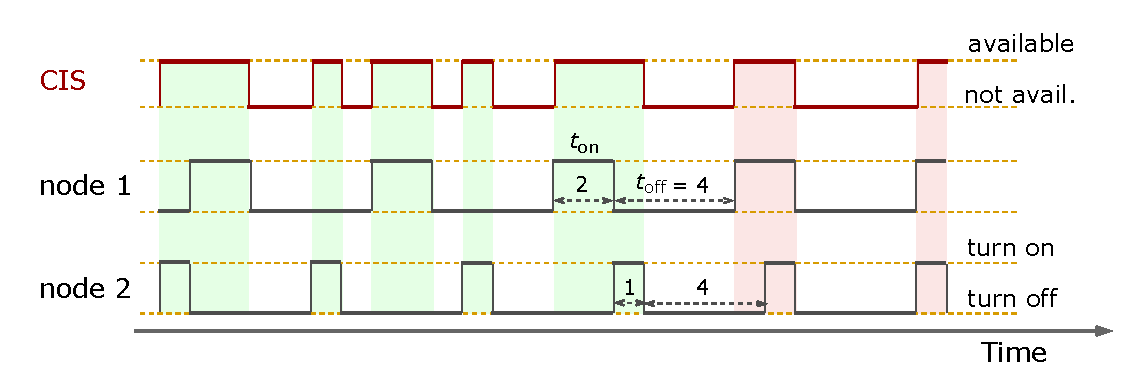
\includegraphics[width=\columnwidth]{figures/cisOntime}
		\caption{A \fullsys's availability is the emerging collective on-time of its intermittent nodes' on-times. The difference between the power cycles leads to a constant relative shift between the nodes duty cycles. This, in turn, causes their on-times to be uniformly distributed on the overall power cycle. The red bars indicate a minimum \sys time span---\sys's nodes are overlapping---whereas the green bars show the maximum time span of the \sys.}
		\label{fig:cisOntime}
\end{figure} 
%
\begin{figure}
		\centering
		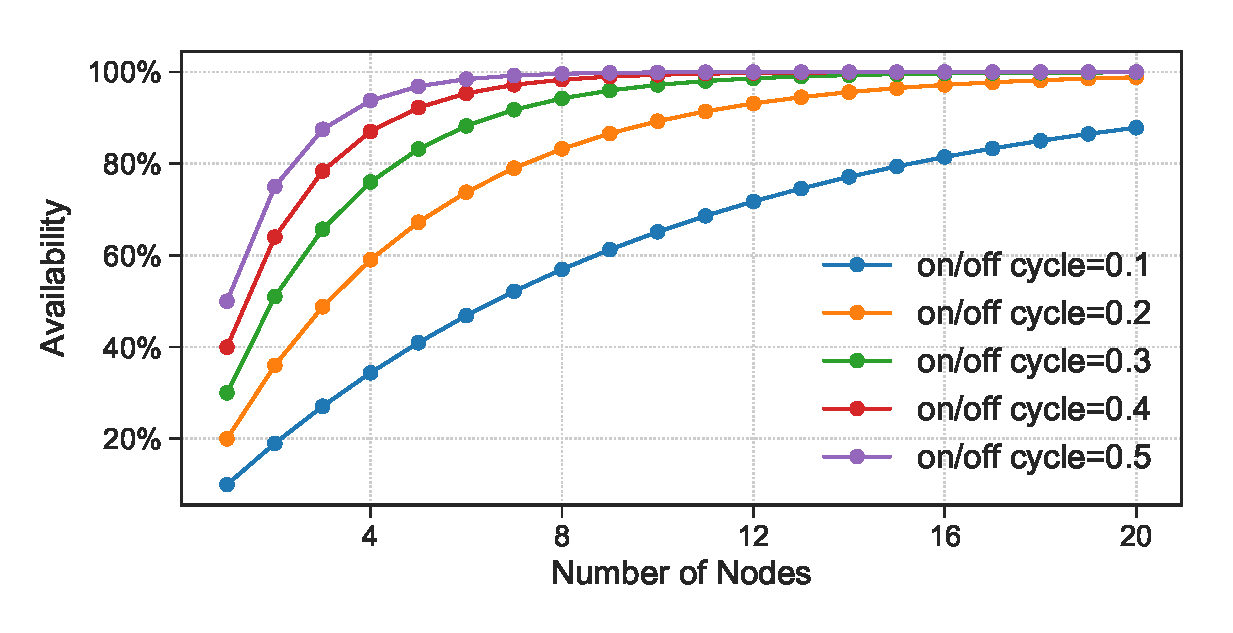
\includegraphics[width=\columnwidth]{figures/cisModel}
		\caption{\fullsys availability percentage for a different number of nodes and different duty cycles. The nodes are uniformly distributed and the \sys on-time evolves, when adding new nodes, according to the equation~\ref{eq:cisModel}.}
		\label{fig:cisModel}
\end{figure} 
%
\paragraph{Implicit on-time division strategy} 
With no information being exchanged between intermittent nodes, the best \sys can do is to uniformly distribute its node's on-times and maintaining this distribution over time. 
The key observation to approach uniform distribution is to ensure that the lengths of the node's power cycles are randomized, avoiding nodes being in lockstep indefinitely.

Let us start by assuming that we have a \sys of two nodes with idealized power cycles and those nodes have the same initial conditions. The availability of this \sys equals $t_\text{on}$ as the nodes are in perfect synchronization (the two nodes wake up and power down together). 
To extend the availability of this \sys, one of the node should
shift its on-time away from the other. If one of the nodes sleeps for $t$\,units of time, then the on-time of this power cycle will be $t_\text{on}+\Delta t$. Consequently, the length of the power cycle itself will be $t_\text{p} + \Delta t $, delaying the next awake time by $\Delta t$.
If the node sleeps only once, then availability of the \sys will equal $\min \left(2\times t_\text{on}| t_\text{on}+\Delta t\right)$

However, if the initial conditions are unknown, then shifting a node's on-time a constant number of times may cause the initially desynchronized nodes to become synchronized, collapsing the \sys's availability instead of extending it. Therefore, a safer option is to \emph{constantly} shift the awake time of the node. In this case, the on-time will shift over the entire power cycle of the other node, spending $\frac{ t_\text{off} }{t_\text{p}}$ and $\frac{ t_\text{on} }{t_\text{p}}$ of the time overlapping with its off-time and on-time, respectively. This behavior is illustrated in Figure~\ref{fig:cisOntime}, where node 1 and node 2 have power cycles of (2,6) and (1,5). Following the time axis from the left to the right, we can observe that the position of the on-time of node 2 is shifted by -1 unit of time relative to the on-time of node 1 after each power cycle of node 1. This implies that the on-times of the two nodes are $\frac{1}{3}$ of the time cluster together and $\frac{2}{3}$ of the time they are apart (from an external event standpoint, the on-times are uniformly distributed over the longest power cycle, as they have the same probability to be anywhere when the event arrives). 
%
If we extend the previous scenario to a \sys of $N$ nodes such that nodes' on-time $t_\text{on}^i \in \{ t_\text{on}^1,t_\text{on}^2,... t_\text{on}^N \}$ and their power cycles $t_\text{p}^i \in \{ t_\text{p}^1,t_\text{p}^2,\text{...} t_\text{p}^N \}$, then we can model the \sys availability as,
%	
\begin{equation}
	A_\text{v}(N) = A_\text{v}(N-1) + \left(1-A_\text{v}(N-1)\right) \times \frac{t_\text{on}^i}{t_\text{p}^\text{max}},
		\label{eq:cisModel}
\end{equation}

where $N \in \mathbb{N}$ and $t_\text{p}^\text{max} = \max\left({ t_\text{p}^1,t_\text{p}^2,\text{...} t_\text{p}^N } \right)$; for the initial case where $N=1$ we define $A_\text{v}(0)\coloneqq 0$. Figure~\ref{fig:cisModel} shows the availability of \sys when $N\in\{1,2,..,20\}$ and nodes' duty cycles $\frac{t_\text{on}}{t_\text{p}}\in\{10\%,20\%,..,50\%\}$.
%
We can conclude from the above discussion that to approach uniform distribution of nodes on-times, the lengths of the power cycles need to be randomized~\footnote{Note that, having power cycles of lengths that are multiples of each other is a very unlikely as nodes' energy buffers are assumed to be of the same size.}. 

The power cycles of energy-harvesting battery-less devices are inherently randomized and different because the power source (ambient energy) is volatile and the harvesters are not perfect devices (notice that, even battery-powered wireless sensor nodes require a synchronization protocol to correct for the drift in their local clocks). Our own measurements on different energy-harvesting devices and different energy sources, i.e., solar and RF, also confirm that the power cycles of intermittent nodes are different and randomized, see Figure~\ref{fig:power_cycles}. Therefore, we expect their on-times to be uniformly distributed (we will challenge our expectation in Section~\ref{sec:evaluation}). 
%
\begin{figure}[t]
		\begin{subfigure}{.49\columnwidth}
			\centering
			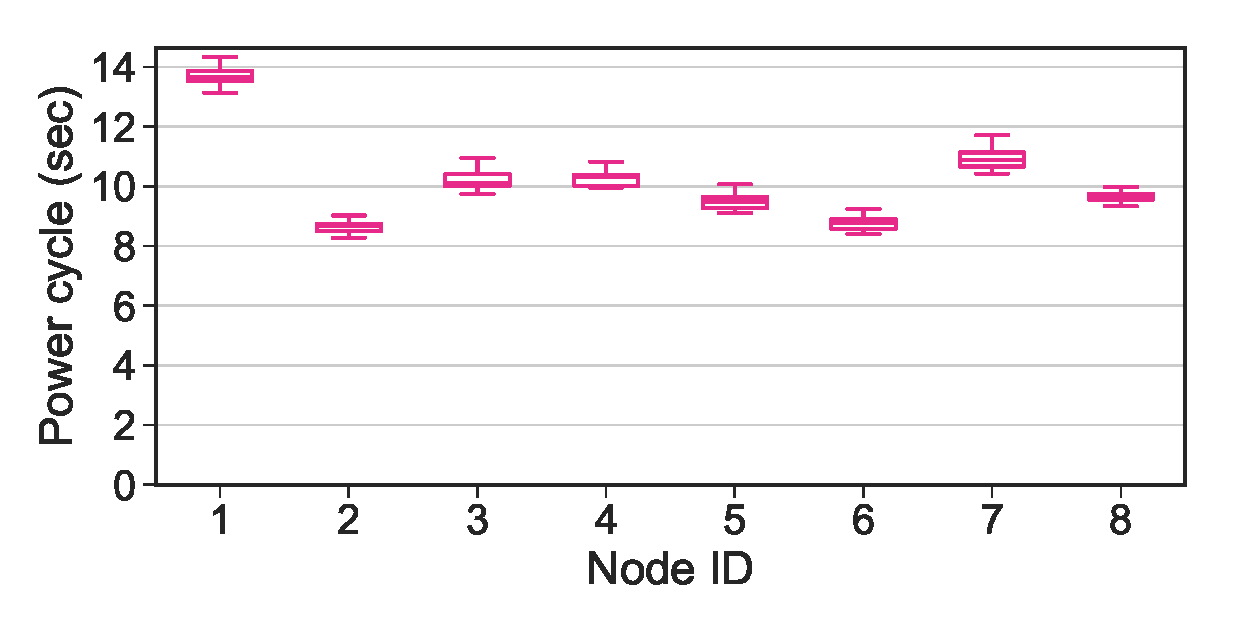
\includegraphics[width=\textwidth]{figures/light_power_cycles_len}
			\caption{Light}
		\end{subfigure}\hfill
		\begin{subfigure}{.49\columnwidth}
			\centering
			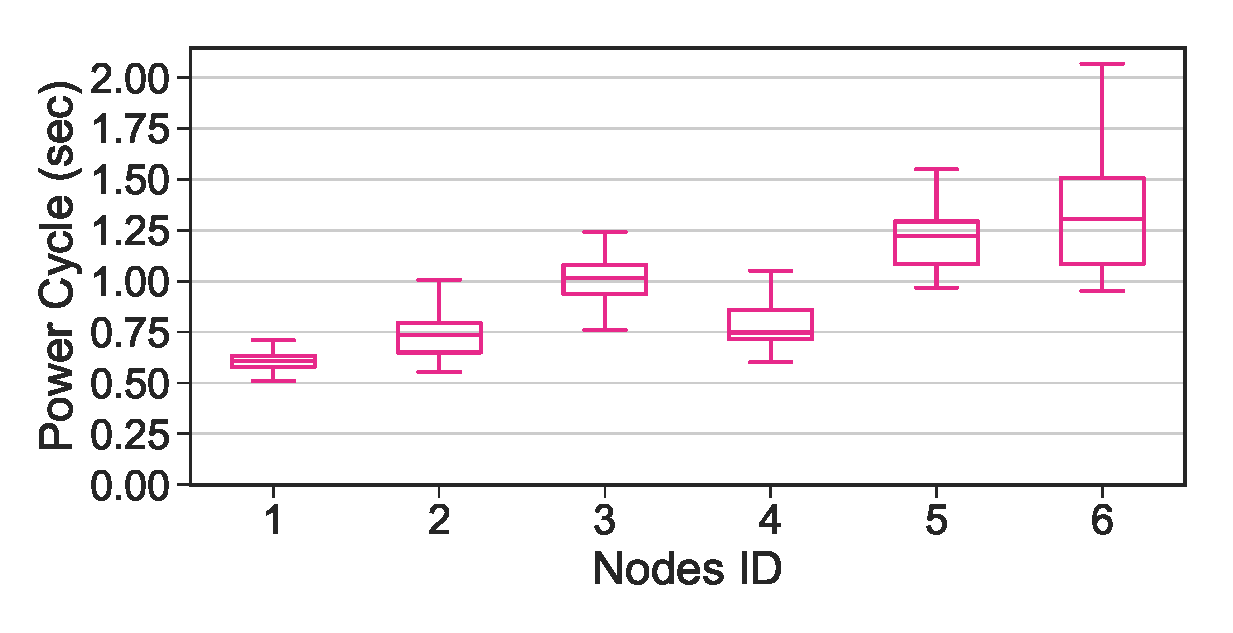
\includegraphics[width=\textwidth]{figures/rf_power_cycles_len}
			\caption{RF}
		\end{subfigure}\hfill
		\caption{Nodes' power cycles length for different energy sources, and different energy buffer sizes.}
		\label{fig:power_cycles}
\end{figure} 
%
\subsubsection{Events classification}
\label{sec:event_classification}
The availability of a \sys is not a single stretched interval: it is a chain of short intervals. Therefore, it is important to classify, from a \sys perspective, which types of events the \sys is best suited for. 
%
\begin{itemize}
\item \textit{Short events}: are events that can be captured using single intermittent node. For example, a spoken word can be seen as a short event if the energy needed to recorded is less than what the energy buffer, i.e., the capacitor, can store.
\item \textit{Long events}: are events that need more energy to be completely captured than what the energy buffer can store. They can be subdivided into three categories: 
	\begin{itemize}
		\item \textit{Simple}: is a long event that can be captured using single intermittent node---capturing part of it is sufficient to obtain all the information of interest---such as the sound produced by the friction between two moving parts of an engine. 
		\item \textit{Burst}: is a group of short events that requires multiple intermittent nodes to be captured such as a command of a few words (e.g., room temperature up).
		\item \textit{Complex}: is a long event that must be fully captured to be recognized. For example, sampling a gyroscope attached to a moving device (e.g., a teeth brush).

	\end{itemize}
\end{itemize}

Based on the above classification, we can argue that designing a \sys for long events is not like designing it for capturing short ones. While capturing a short event may require continuous \sys availability, capturing a long simple event that is longer than the power cycle $t_\text{p}$ does not require extending the availability of a single intermittent node. Furthermore, capturing a long complex event may require data fusion and processing that require the \sys{}s' nodes to communicate the raw data to a more powerful node, which may lead to significant overhead. However, this paper focuses on short and long bust events as they cover a wide range of applications (e.g., voice-controlled human-object interface). 
%ToDo what about the long smpile event (it is a relax version of the problem of capturing short event, i.e., less less stricked availability is required)

\subsubsection{Effective Availability}
%
\begin{figure}
		\centering
		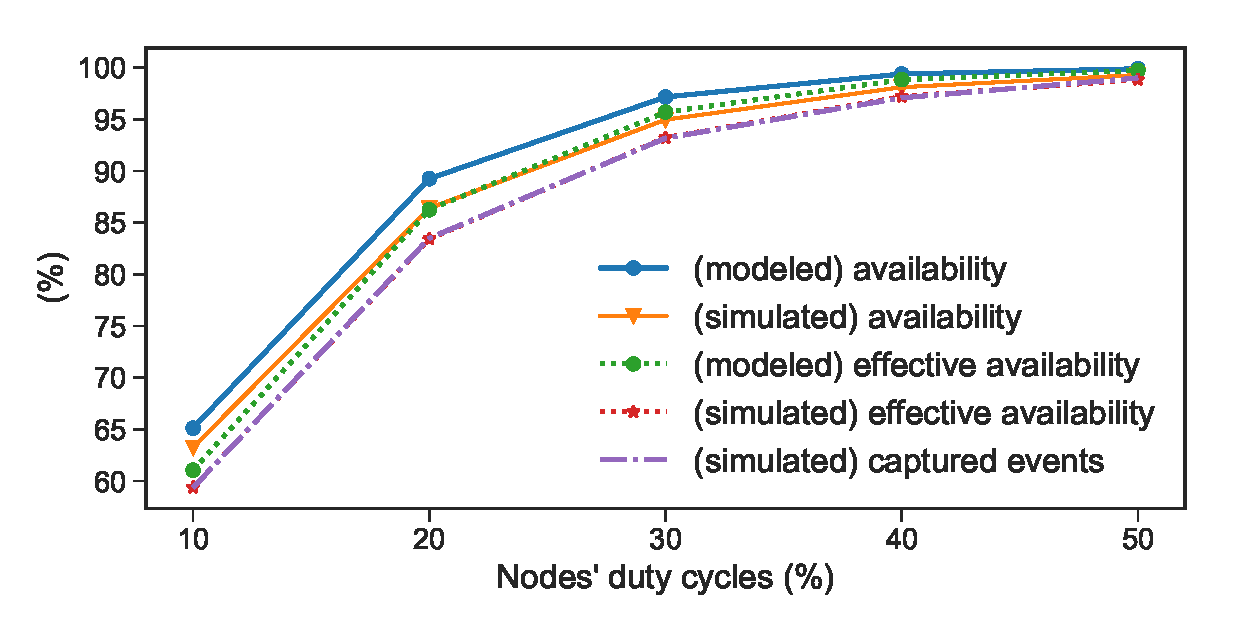
\includegraphics[width=\columnwidth]{figures/effective_availability}
		\caption{Simulating the availability, the effective availability, and successfully captured events of a \sys of 10 nodes with a node duty cycle $\in \{10\%, 20\%,...,50\%\}$.}
		\label{fig:cis_simulation}
\end{figure}
%
Approaching continuous availability does not mean that a \sys can successfully capture all events. It can happen that an event is being only partially captured by one or more nodes, which may lead to unsuccessful event detection. Therefore, it is important to specify the effective availability of a \sys that leads to a successful event capturing (which we assume leads to successful sensing). 

\paragraph{polling-based Sensing}
Let us assume that we have a \sys of a single intermittent node monitors a short event of length $t_\text{e}$. For capturing the entire event, the event has to arrive within the interval, $t_\text{on} - t_\text{e}$, which we call, the effective on-time of an intermittent node.
Therefore, the effective availability of a \sys of $N$ nodes is the joined effective on-times of the underlying intermittent nodes, which can be modeled as,
%
\begin{equation}
		A_\text{v}(N) = A_\text{v}(N-1) + \left(1-A_\text{v}(N-1)\right) \times \frac{t_\text{on}^i - t_\text{e}}{t_\text{p}^\text{max}},
		\label{eq:cisSenseModel}
\end{equation} 
%

\paragraph{Event-driven Sensing}
An intermittent sensor has a limited energy budget per power cycle. When it is tasked with a polling-based sensing activity, its energy consumption, generally, switches between two levels: zero when charging and maximum when it activates its microcontroller for data acquisition and processing (Note that we assume that the microcontroller is the dominant energy consumer module of a node). However, in event-based sensing, a node puts its microcontroller into low-power mode and waits (or listens) for an external event to wake up the microcontroller. For example, in our prototype, a voice-controlled command recognizer, we exploit the microphone's wake-on-sound feature to send an interrupt to the microcontroller, which will then start recording the sound samples from the microphone. 
This wake-on-event style of operation is important as the minimal energy consumption during sleep significantly prolongs the period during which an event can be handled (for example, our prototype consumes 7 times less energy during sleep compared to being active).
To model the effective \sys availability when it is tasked with event-based sensing the change in energy consumption between the sleep and active mode must be taken into account. Since the event itself times when the node changes its energy consumption, we can model the effective availability as,
\begin{equation}
		A_\text{v}(N) = A_\text{v}(N-1) + \left(1-A_\text{v}(N-1)\right) \times \frac{t_\text{on}^i - (t_\text{e} \times\frac{e_\text{a}}{e_\text{s}}) }{t_\text{p}^\text{max}},
		\label{eq:cisEventSenseModel}
\end{equation}

where $e_\text{a} and e_\text{s}$ are the energy consumption at active and sleeping modes, respectively.
%
\subsubsection{Simulation}
To do a first sanity check on our models, we simulated $10^5$ power cycles of a \sys of 10 nodes (Figure~\ref{fig:cis_simulation}). The duty cycles of the nodes range from $10\%$ to $50\%$, while the event length is fixed at $3\%$ of the power cycle length, $t_\text{p}$. The on-times and events arrivals were uniformly distributed over the power cycles. 
The results clearly confirm our models and support our argument about the distinction \sys's availability and effective availability. The importance of this distinction is a function of the value $\frac{t_\text{e}}{t_\text{on}}$; observe the difference between availability and effective availability when nodes' duty cycle is $10\%$ and $50\%$.
%
%
\subsection{Environment}
Ambient energy controls the availability of a \sys's nodes.  Consequently, it also controls their collective response to external events. When it rises, it extends nodes' on-times. Extended on-times may cause node's power cycles to be synchronized on events arrival, compromising the \sys's overall availability. To overcome this problem the \sys's nodes must be power-state aware and able to estimate the number of active nodes in the \sys.
%
\subsubsection{Power States}
\label{sec:power_state}
A \sys can experience a wide range of ambient power intensities. For example, a solar-powered \sys may harvest no energy at night, modest energy from artificial light, and abundant energy from direct sunlight.  Generally, we can identify four different \sys powering states: 
\begin{itemize}
		\item \textit{Targeted power state}---These are the powering conditions that a \sys is designed for. In these  conditions, the \sys should work intermittently and have sufficiently randomized power cycles to uniformly distribute its intermittent nodes on-times and meet the desired availability (Figure~\ref{fig:cisModel}). In general, the targeted powering conditions should be near worst energy harvesting conditions to ensure that the system is properly functioning for the majority of the time.
		\item \textit{Under-targeted power state}---Ultimately, the ambient energy is an uncontrollable power source, and it is not hard to imagine scenarios where a \sys will be under-powered or even comes to complete and long power down (for example, a solar \sys will come to a perpetual power down in the darkness). In general, for under-targeted energy conditions, the \sys behavior can be considered as undefined.
%
\begin{figure}
		\centering
		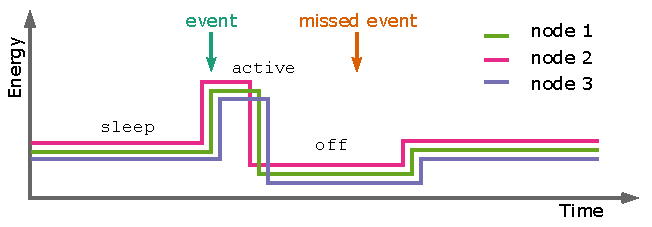
\includegraphics[width=\columnwidth]{figures/hibernating_power_state}
		\caption{\fullsys is in a hibernating power state when the energy harvesting rate approximates the energy consumption rate at the sleeping (or low-power) mode. In this state, the intermittent nodes lose the randomization in their power cycles. Thus, all the nodes capture the same event and power down shortly after missing the subsequent ones. Consequently, the \sys senses intermittently and does not take advantage of its redundant intermittent nodes to approach continuous sensing.}
		\label{fig:noRand}
\end{figure} 
%
		\item \label{it:hibernating} \textit{Hibernating power state}---In event-based sensing scenarios, the intermittent nodes of a \sys sleep in low-power mode waiting for an external event to wake them up. If the energy conditions are relatively higher than the targeted conditions, the nodes may not die and sustain their sleeping power consumption. This will cause them to synchronize their wake-ups on the first incoming event and their power down as the event capturing process depletes their energy buffers quickly. Consequently, the \sys may miss the next incoming events (specially if the events happens to arrive in bursts) causing it to sense intermittently instead of continuously, see Figure~\ref{fig:noRand}. 
		%
		\item \label{it:continuous} \textit{Continuous power state}---Under direct mid-noon sun a tiny solar panel may provide sufficient power to run a sensor node continuously. In such conditions, the \sys will sense continuously without the need for randomization. Therefore, the job of a single node will be repeated $N$ times, and instead of sending a single message to a battery-powered or tethered sink---to push the data to the Internet---$N$ identical messages will be sent.
		These messages will collide as they are sent at about the same time, causing the information to be lost; if they arrive, however, they -except the first one- will waste energy of the sink as they carry the same information.  
		 % at about the same time causing them to collide or waste energy as they replicated the same information that has been delivered by the first message. 
				
\end{itemize}
%
The inefficiencies highlighted in the hibernating and continuous power states can be mitigated by enforcing randomization on the response of intermittent nodes 
% (Figure~\ref{fig:rand})
: when a node is woken up by an external event it responds to that event with a certain probability. However, if the randomized response is enforced all the time, then the \sys will have a lower probability of catching events during the targeted energy conditions state. Therefore, the \sys has to distinguish between the targeted and above-targeted energy conditions and randomize its response only during the hibernating and continuous power states. 

Choosing a fix response probability is an inefficient way of dealing with the over-powering problem as the number of active intermittent nodes at a given moment is a function of the total number of intermittent nodes and the power intensity at that time. Therefore, efficient randomization requires intermittent nodes to estimate the number of active nodes at the event arrival moment (which is discuss it next) and respond proportionally.

\subsubsection{Intermittent Timing}
\label{subsec:interTimer}
%
\begin{figure}[t]
		\centering
		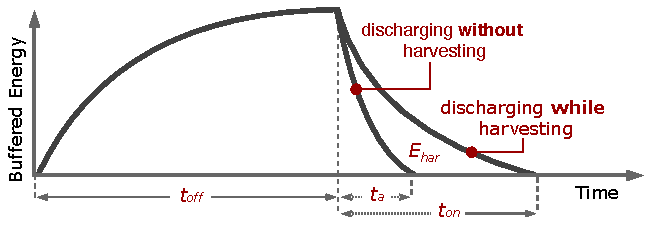
\includegraphics[width=\columnwidth]{figures/softwareClock}
		\caption{The difference in the time of discharging the energy buffer---a node's on-time---when an energy-harvesting device is allowed to charge while operating, and when it is not allowed.}
		\label{fig:softwareClock}
\end{figure} 
\begin{algorithm}[t]
	\captionof{algorithm}{off-time estimation}
    \label{algo:offTime}
    \small
    \begin{algorithmic}[1]
		\State \Call{$f_\text{reboot}$}{$u$} $= u{+}{+}$ \Comment{power reboot counter}
			\State $i \leftarrow $ \Call{$f_\text{reboot}$}{$i$} \Comment{$i$ is a persistent variable} \label{lin:i}
		\State $E_\text{buf}$ \Comment{Size of energy buffer}
			\State $t_a$ \Comment{time of discharging $E_\text{buf}$ at load $a$, no harvesting}\label{lin:ta}
		\State$ t_{i} \leftarrow x $ \Comment{timing every $x$ power cycles}
		%
		\If{$(i\mod t_{i})=0$}
		    \State $i=0$
			\State \Call{$f_\text{load}$}{$a$} \Comment{set node load to $a$ } \label{lin:fixedLoad}
			\State \label{lin:ontime} $t_\text{on} \leftarrow$ \Call{$t_\text{pers}$}{\null} \Comment{persistent infinite loop}\label{lin:ton}
		\EndIf
		\If{$i=1$}
			\State \label{lin:deltat}$\Delta{t} = t_\text{on}-t_a$  \Comment{time difference due to charging} \label{lin:td}
			\State \label{lin:ehar}$E_\text{har} \leftarrow (E_\text{buf}\div t_a)\times\Delta{t}$ \Comment{harvested energy}
			\State $P_\text{in} \leftarrow E_\text{har}\div{t_\text{on}}$ \Comment{incoming power} \label{lin:pin}
			\State \label{lin:offtime}$t_\text{off} \leftarrow E_\text{buf}\div P_\text{in}$ 
		\EndIf
	\end{algorithmic}
\end{algorithm}
%
Timing is a key building block of sensing systems. It is, however, missing on intermittent nodes unless an additional dedicated (RC-based) timer is added to them~\cite{hester2017timely}. Here we would like to propose an alternative that does not require additional hardware. This alternative does not only enable time estimation but also ambient energy richness, which is very important for estimating the number of a node's active neighbors. But, \textit{how a node can time its own on/off cycle?}

Intermittent nodes fail abruptly; therefore, a persistent timer is needed. A simple way to emulate persistent timer is by using a persistent counter, or sampling the volatile built-in timers of the microcontroller and save the obtained values in the non-volatile memory. To estimate the off-time, $t_\text{off}$ in Figure~\ref{fig:softwareClock}, a node needs to determine the incoming power (harvesting rate). The average harvesting rate can be induced from the on-time as follows.
%
The node measures its on-time while harvesting, see $t_\text{on}$ in Figure~\ref{fig:softwareClock}, and compares it to the time required to drain the energy buffer \emph{without} charging, see $t_\text{a}$ in Figure~\ref{fig:softwareClock}. The additional on-time, $\Delta t$, is the result of the energy accumulated while executing. 
%
If $t_\text{on}$ and $t_\text{a}$ are measured on the same load---thus, they have the same power consumption---then the amount of the energy harvested while the device is on can be calculated as in Line~\ref{lin:ehar}, Algorithm~\ref{algo:offTime}. And, the average input power can be found as in Line~\ref{lin:pin} that, in turn, enables the node to estimate its own $t_\text{off}$ (Line~\ref{lin:offtime}).
Since calculating the off-time requires constant load, the sensor cannot run arbitrary code during time measurement. Therefore, the sensor needs to sacrifice a certain percentage of its power cycles for time measurement, Line~\ref{lin:i}-\ref{lin:ton}. Once the on-time and off-time are found the node's power cycle is determined.

\subsubsection{Nodes overlapping}
\begin{figure}[t]
		\centering
		\begin{subfigure}{.49\columnwidth}
			\centering
			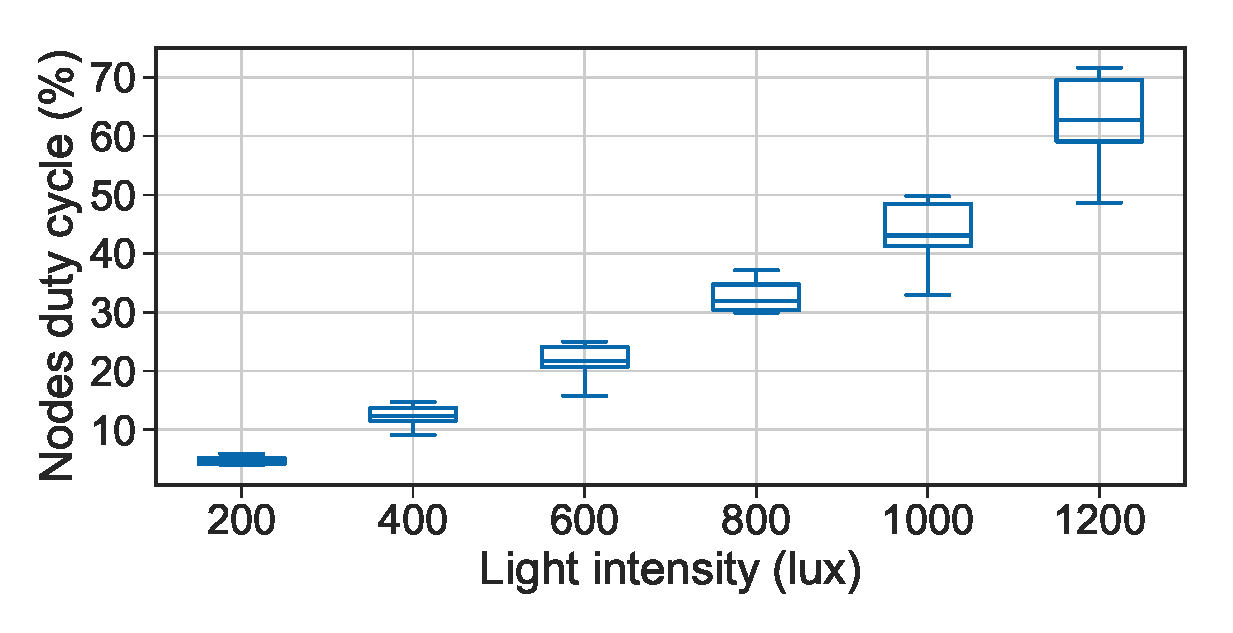
\includegraphics[width=\textwidth]{figures/cis_dutyCycle}
			\caption{Light}
		\end{subfigure}\hfill
		\begin{subfigure}{.49\columnwidth}
			\centering
			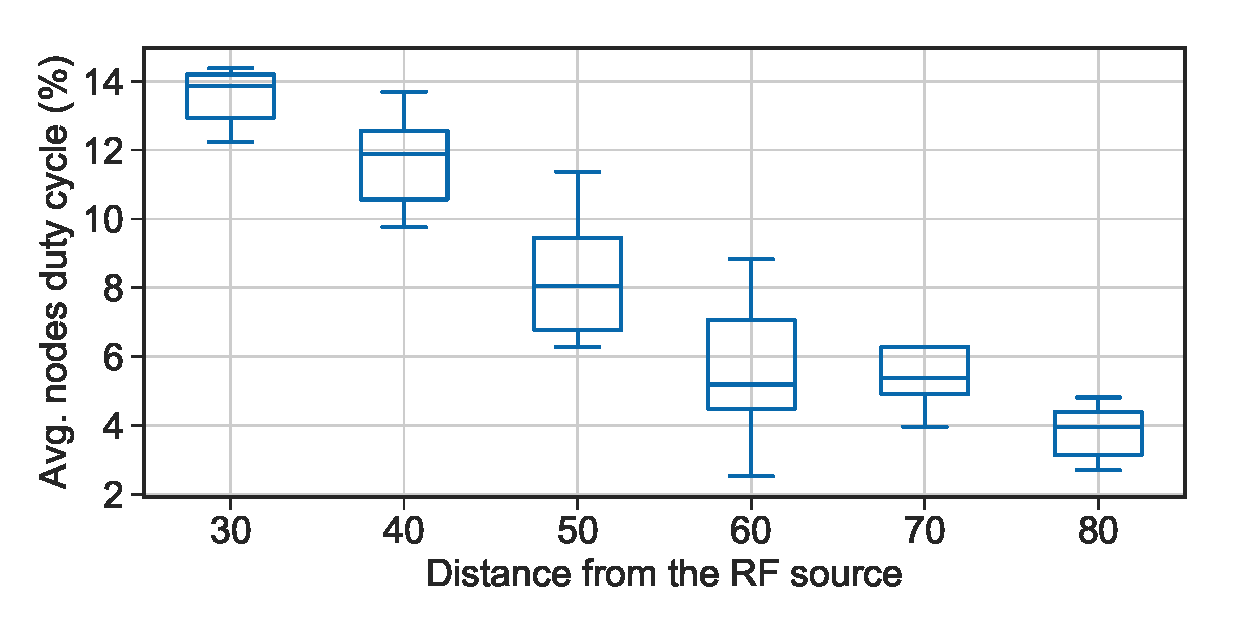
\includegraphics[width=\textwidth]{figures/rf_cis_dutyCycle}
			\caption{RF}
		\end{subfigure}\hfill
		\caption{The average duty cycles of 8 solar-powered and 6 RF-powered intermittent nodes for different ambient energy sources and energy intensities. In general, the average duty cycle of a node is a good indicator of the average duty cycle of \sys's nodes.}
		\label{fig:cis_nodes_dutyCycle}
\end{figure} 

\begin{table}
		\centering
		\caption{Measuring intermittent nodes overlapping of a \sys of 8 intermittent nodes for different light intensities.}
		\begin{tabular}{lll}
				\hline
				light (lux) & $N_\text{active}$ & std    \\
				\hline
				300	                  & 1.01 & 0.85   \\
				500                   & 1.63 & 0.98   \\
				800                   & 2.88 & 1.50   \\
				1200                  & 5.05 & 1.08   \\
				\hline
		\end{tabular}
		\label{tab:clusters}
\end{table}
% In order for a node to estimate the number of active nodes at a given moment, first, it has to know the total number of nodes ($N$) in its \sys, which we assume to be known to the nodes before deployment. Second, this analysis is built on the observation that a node's on-time is a good indicator about the on-times of other nodes in the \sys, see Figure~\ref{fig:cis_nodes_dutyCycle}. A node can measure its on-time $t_\text{on}$ and off-time $t_\text{off}$ using  Algorithm~\ref{algo:offTime} (or an external dedicated timer~\cite{hester2017timely}). 

Now, a \sys's node has all the information needed to estimate the number of active nodes in its \sys. Namely, it knows

In order for a \sys's node to estimate the number of active nodes at a given moment, it needs to determine the following information: 
\begin{enumerate*}[label=(\roman*)]
 \item the size of the \sys it belongs to, which is a constant value that can be loaded to the memory; 
 \item its own $t_\text{on}$ and $t_\text{off}$; and 
 \item how the \sys's nodes' on-times are distributed, Model~\ref{eq:cisModel}.
\end{enumerate*}
% Notice that, on/off times of a \sys's node can be used to estimate other \sys's nodes' on/off times.
% This is intuitively valid as the nodes have the same energy buffer size and are expose to the approximately the same energy conditions~\footnote{}. 
Figure~\ref{fig:cis_nodes_dutyCycle} shows the average power cycles of solar- and RF-powered nodes.
We can conclude from these measurements that a node power cycle approximates other \sys's nodes power cycles.
This observation can be generalized by considering that the nodes of a \sys are assumed to have the same energy buffer size and they are in a close proximate, and therefore, they are expose to roughly the same energy conditions (this should not be confused with argument about the emerging uniform distribution of nodes' on-times as this distribution appears due to \emph{small} differences between the power cycles).  

Now, a node can estimate the maximum time span ($t_\text{max}$) of its \sys, which is the total duration of the nodes' on-times when they are aligned next to each other, as follows
\begin{equation}
t_\text{max} = N\times t_\text{on}.
		\label{eq:max_time}
\end{equation}
Then, from Equation~\ref{eq:cisModel}, the node calculates the \sys availability ($t_\text{on}(N)$). As we argued in Section~\ref{subSec:availability}, nodes on-times are uniformly distributed over the longest power cycle, $t_\text{p}^\text{max}$. Thus, the overlapping on-time is also uniformly distributed. Then, the node can calculate the average number of active intermittent nodes $N_\text{active}$ using the following formula,
\begin{equation}
	N_\text{active} = \frac{t_\text{max}}{t_\text{p}^\text{max}\times A_\text{v}(N)}.
	\label{eq:active}
\end{equation}
and choose the proper randomization factor. If a second event, however, happens shortly after the first one, a node needs to update $N$ as follows, 
$$
N = N - (N_\text{active}-1)
$$
the $-1$ is because the node itself decided not to react on the first event. 

Table~\ref{tab:clusters} shows the average number of overlaps of an 8-nodes \sys for different light intensities. These measurements validate that nodes overlapping time is uniformly distributed over the \sys on-time. For example, at $\SI{1200}{lux}$ an individual node of our \sys has a duty cycle of $\approx$\,62\%. If we multiply it by the number of nodes (Equation~\ref{eq:max_time}) we get about 500\%. Figure~\ref{fig:cisModel} indicates that a \sys with eight nodes of duty cycles above 50\% has near 100\% availability. From equation~\ref{eq:active}, we find that the expected number of clustered nodes is 5 which is what Table~\ref{tab:clusters} also shows. 








































